\chapter{Development of a WIDS}

\section{Overview}

As described in section \ref{sec:wids_definition} the purpose of a wireless intrusion detection system is to detect a malicious client in a network. This chapter shows a concept of a hybrid WIDS which is capable of identifying different threats in a WLAN. Appendix \ref{sec:implementation} shows the tools which are used to create the WIDS and the test environment.

Possible threats include rogue APs, unknown clients, association and disassociation flood attacks. First, the goals of the WIDS are discussed. Then, design details like the classification of the traffic in a network and the process of feature selection is shown. Additionally, an algorithm which finds the best feature set for every problem that needs to be solved is described.

\section{Goals}

The goal of the tool being developed is to create a hybrid WIDS which on the one hand uses well known techniques to detect threats like rogue APs and malicious users. On the other hand it uses a neural network to learn how to identify different wireless threats like association and disassociation floods. The following list shows the main goals of the tool:
\vspace{-0.5em}
\begin{itemize}
	\item It should be possible to use it in every WLAN without worrying about the type of encryption used
	\item Use a neural network to detect association and disassociation flood attacks after a learning phase
	\item The system should be able to react to changes in the characteristics of the network. That means in other words that the WIDS realises when the properties, like the average amount of traffic or the number of connected clients in a network, change
	\item Use white lists to detect rogue APs and malicious clients
	\item It has to be able to receive the input values either from a pcap file\footnote{See glossary} or directly from a capturing NIC. The idea is to perform learning by using a previously stored pcap file. After the learning phase is finished the WIDS starts to capture and analyse packets for intrusion detection

\end{itemize}

\section{Design}

The following sections explain design details of the WIDS, its preprocessor and the process of finding the best feature set for the neural network.

\subsection{WIDS}
\label{sec:design_wids}

The overall design of the WIDS follows the suggested structure presented in section \ref{sec:ids_structure}. Figure \ref{wids_dataflow} shows the four components used and the data flow in the WIDS.

\begin{figure}[htbp]
	\begin{center}
		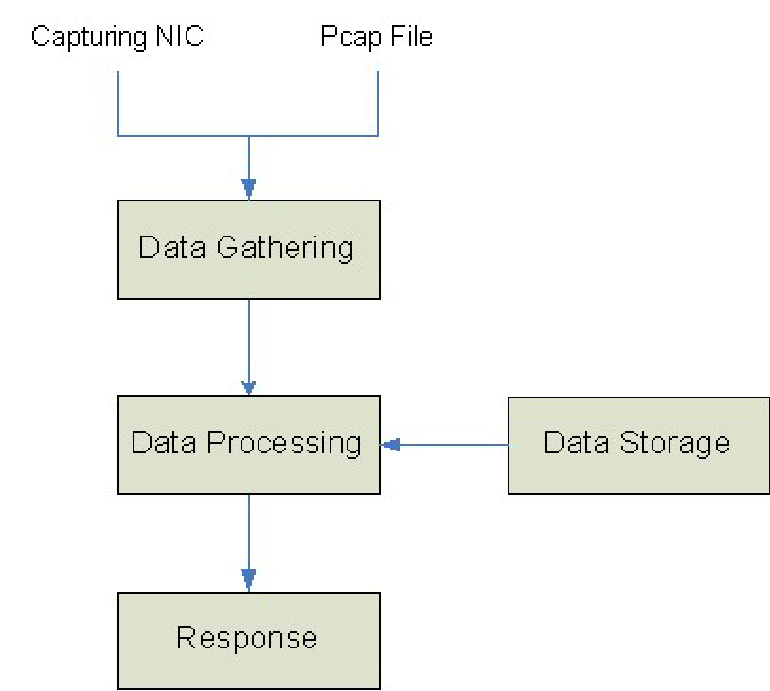
\includegraphics[width=0.7\columnwidth]{graphics/WIDS_structure}
	\end{center}
	\vspace{-1em}
	\caption{Components and data flow in the WIDS}
	\label{wids_dataflow}
\end{figure}

{\em {\bf Data Gathering}}

This component is used to receive data either from a previously stored file or directly from a capturing NIC. The data gathering component forwards the data directly to the data processor.

\pagebreak

{\em {\bf Data Processing}}

The core of the data processing component is a neural network. After training it is capable of identifying association and disassociation flood attacks. It uses the backpropagation learning algorithm described in section \ref{sec:backpropagation}. In addition to the neural network the processor also identifies rogue APs and unknown clients by comparing the content of the white lists created by a preprocessor (described in section \ref{sec:preprocessing}) with the packets received from the data gathering component.

{\em {\bf Data Storage}}

After the training phase this component stores information about a trained neural network. Stored information includes all weights of the network and the {\em scaling values}\footnote{A scaling value specifies the maximum amount of packets with a certain type/subtype that occur in a two second time slot} received. That makes it possible to

\begin{itemize}
    \item create a trained neural network by assigning the stored weight values to the connections between neurons. As a consequence no training phase needs to be done
\vspace{1em}

	\item perform the training phase in several steps. After one training phase is finished it is possible to continue training the network with additional data. This is an important point for the WIDS to be able to react to changes in the network behaviour. The training of the neural network can continue after the initial learning phase is finished by using the data coming directly from the capturing NIC
\end{itemize}

{\em {\bf Response}}

This component is responsible for informing the operator of a WLAN about ongoing threats in the network. The WIDS prints an alert message on the screen.

\subsection{Preprocessing}
\label{sec:preprocessing}

Before the WIDS can be trained several preprocessing steps need to be performed. In order to be able to perform these steps the preprocessor requires a pcap file with normal traffic and one or more files which contain flood specific traffic.

The preprocessor creates white lists for rogue AP and malicious user detection. These lists store the BSSID of every network and the MAC address of every client found inside the normal traffic file.

It addition to the white lists the preprocessor creates additional pcap files (named {\em relevant files}) which are used by the neural network in order to learn the characteristics of different flood attacks. A prototype implementation of the WIDS, which used only the normal traffic file and the flood files to learn, showed, that the neural network does not succeed in learning the characteristics of a flood attack. The reason for that is that association and disassociation packets occur very rarely compared to other packets. As a consequence the neural network would learn too slowly. The relevant files are created out of the normal traffic files and contain only those data packets with the type and subtype field that also occur in the respective flood file.

As soon as these preprocessing steps are finished the network can be trained. The training requires a pcap file with normal traffic, all relevant files and all files which contain flood specific traffic. 

\subsection{Features}

"Since the ability to identify the important inputs and redundant inputs of a classifier results in reduced problem size, faster training and possibly more accurate results, it is critical to be able to identify the important features of network traffic data for intrusion detection in order for the IDS to achieve maximal performance" \cite{nn_features}. That means in other words that the quality of the neural network does not solely depend on the number of hidden layers or neurons used but also on the input features\footnote{A feature is for example the amount of traffic sent to a client or the number of connections coming from the same host in a specified period of time} chosen.

\subsubsection{Feature Selection}
\label{sec:features}

The group of features used as inputs for the neural network is divided into two different sections:

\begin{description}
    \item[Time irrelevant features:] This type of features includes all values that are available by dissecting one single frame. These features do not consider the time aspect. All values are converted to binary values and then given to the neural network.

	\begin{itemize}
	    \item Type field
		\item Subtype field
		\item Retry field
	\end{itemize}

    \item[Time based features:] This type of features takes the period of time that passed since a specific event that happened in the past into account. The WIDS uses two features of this type:

	\begin{itemize}
		\item The number of frames with a certain type and subtype in the past two seconds. This feature is needed to detect association and disassociation floods. The higher this number is the more probable it is that an attack occurs. When given to the neural network this value is scaled from $0$ to $1$ by using the scaling value as divisor. In case the resulting value is bigger than $1$ it is set to $1$. This formula is written as

\begin{equation}
\frac{number\ of\ same\ packets\ in\ the\ past\ two\ seconds}{scaling\ value\ of\ that\ packet\ type}
\end{equation}
\vspace{-0.5em}
		\item The number of disassociations of legitimate clients in the past two seconds. This feature is needed due to the fact that a disassociation flood is harmless in case the source address of the packet is never used in the network. For that reason this feature is needed which checks for packets with a source address of legitimate clients. Again, when given to the neural network this value is also scaled from $0$ to $1$ by using the maximum number of legitimate clients as divisor. This formula is written as

\begin{equation}
\frac{number\ of\ disassociations\ in\ the\ past\ two\ seconds}{maximum\ number\ of\ legitimate\ clients}
\end{equation}


	\end{itemize}

\end{description}

\subsubsection{Performance Based Ranking Method}

The following algorithm describes a technique to find the best feature set for a specific problem. It was taken and adopted from \cite{nn_features}. Depending on the results obtained this algorithm classifies a feature either as {\em important}, {\em secondary} or {\em unimportant}.

\setlength{\fboxsep}{1em}
\begin{center}

\fbox{\begin{minipage}{250pt}
\begin{enumerate}
	\addtolength{\itemsep}{-1.5ex}
    \item Create the training and testing set
	\item Remove one feature of the neural network
	\item Train the neural network using the training set
	\item Calculate the accuracy using the testing set
	\item Rank the importance of the removed feature according to the rules shown below
\end{enumerate}
\end{minipage}}

\end{center}

The following list shows the rules which rank the importance of one particular feature:

\begin{itemize}
	\addtolength{\itemsep}{-1.5ex}

    \item If $a$ decreases and $r$ increases and $e$ decreases: $f$ is important
	\item If $a$ decreases and $r$ increases and $e$ increases: $f$ is important
	\item If $a$ decreases and $r$ decreases and $e$ increases: $f$ is important
	\item If $a$ unchanges and $r$ increases and $e$ increases: $f$ is important
	\item If $a$ unchanges and $r$ decreases and $e$ increases: $f$ is secondary
	\item If $a$ unchanges and $r$ increases and $e$ decreases: $f$ is secondary
	\item If $a$ unchanges and $r$ decreases and $e$ decreases: $f$ is unimportant
	\item If $a$ increases and $r$ increases and $e$ decreases: $f$ is secondary
	\item If $a$ increases and $r$ decreases and $e$ increases: $f$ is secondary
	\item If $a$ increases and $r$ decreases and $e$ decreases: $f$ is unimportant
\end{itemize}

where

\begin{itemize}
	\addtolength{\itemsep}{-1.5ex}

    \item $a$ is the accuracy of the result
	\item $r$ stands for the training time
	\item $e$ stands for the testing time
	\item $f$ is the feature that was removed before training

\end{itemize}

\subsubsection{Neural Network}

In addition to the input features there exist other properties which can improve the performance of the WIDS. The network based features describe the structure and properties of the neural network itself. All features presented in this set can be modified for every type of problem. Section \ref{sec:test_nn} shows the process of finding the best values for each of these features.

\begin{itemize}
	\addtolength{\itemsep}{-1.5ex}
    \item Initial weight values
    \item Number of hidden layers
    \item Number of neurons in each hidden layer
    \item Learning rate
    \item Appearance of the sigmoid function
\end{itemize}

\subsection{Classification}

Normal traffic in a wireless network has specific properties like the average number of connections to an AP or the amount of traffic sent over the network. Whenever a cracker launches an attack on a network these properties change. As an example a network could have 50 connected clients. When a malicious user would start a disassociation flood attack he would send a large amount of packets of the same type in a short period of time. In a network with legitimate users this would generally not happen.

The traffic in a wireless network is classified into three different groups. These groups are needed so that the WIDS can tell what kind of attack is currently threatening the network.

\begin{description}
    \item[Normal traffic:] This type identifies normal traffic without the occurrence of any attack
	\item[Association flood:] This type identifies an association flood. This traffic is characterised by a large amount of association frames in a short period of time
	\item[Disassociation flood:] This type identifies a disassociation flood. This traffic is characterised by a large amount of disassociation frames coming from legitimate clients in a short period of time
\end{description} 

\chapter{Tests and Results}

\section{Introduction}

This chapter explains the results obtained by the WIDS. At the beginning, the  configuration parameters for the neural network which is used in the WIDS are figured out. Afterwards, the WIDS is trained and tested by using different pcap files. Finally, the results are discussed and possible improvements are shown.

\section{Neural Network}
\label{sec:test_nn}

\begin{description}
	\item [Initial weight values:] These values are especially important whenever a neural network is used which is trained by using a small amount of training data or training cycles. Figure \ref{error_weights} displays the error rates of three training cycles performed one after another. The network configuration stays the same for all three tests except that the weight values change since they are initialised randomly.

\begin{figure}[htbp]
	\begin{center}
		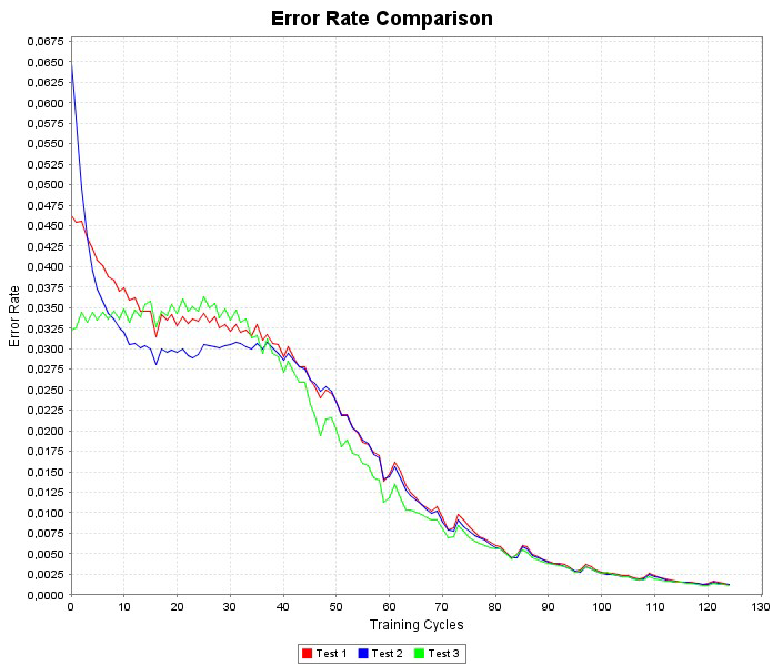
\includegraphics[width=0.7\columnwidth]{graphics/Error_time}
	\end{center}
	\vspace{-1em}
	\caption{A comparison using different initial weight values}
	\label{error_weights}
\vspace{1.5em}
\end{figure}

The result is that all calculated error rates differ in the first 100 training cycles. As it turns out after a training phase that is long enough all error rates conform the each other.
\pagebreak

\item [Number of hidden layers:] One feature that affects the time needed to train the neural network is the number of hidden layers. In this test the number of neurons in each hidden layer is set to the number of input nodes. Tests show that an increasing number of hidden layers raises the time needed to train the network but does not increase the quality of the resulting network.

Each test is performed with 10.000 training cycles. The result is shown in table \ref{train_layers} and figure \ref{error_hidden}. In addition to the amount of time needed, the number of training cycles to train the network also increases.

\begin{table}[htbp]
	\vspace{1.5em}
	\begin{center}
		\begin{tabular}{|l|l|l|}
		\hline
		\bf{Hidden layers}&\bf{Time needed}&{\bf Error rate}\\
		\hline
		1&5.658 sec&1.23151*$10^{-8}$\\
		\hline
		2&10.756 sec&2.13083*$10^{-8}$\\
		\hline
		3&15.602 sec&1.65828*$10^{-8}$\\
		\hline
		4&20.459 sec&3.89512*$10^{-8}$\\
		\hline
		\end{tabular}
	\end{center}
	\vspace{-1em}
	\caption{Resulting time and error when using 1, 2, 3 and 4 hidden layers}
	\label{train_layers}
\end{table}

\begin{figure}[htbp]
	\begin{center}
		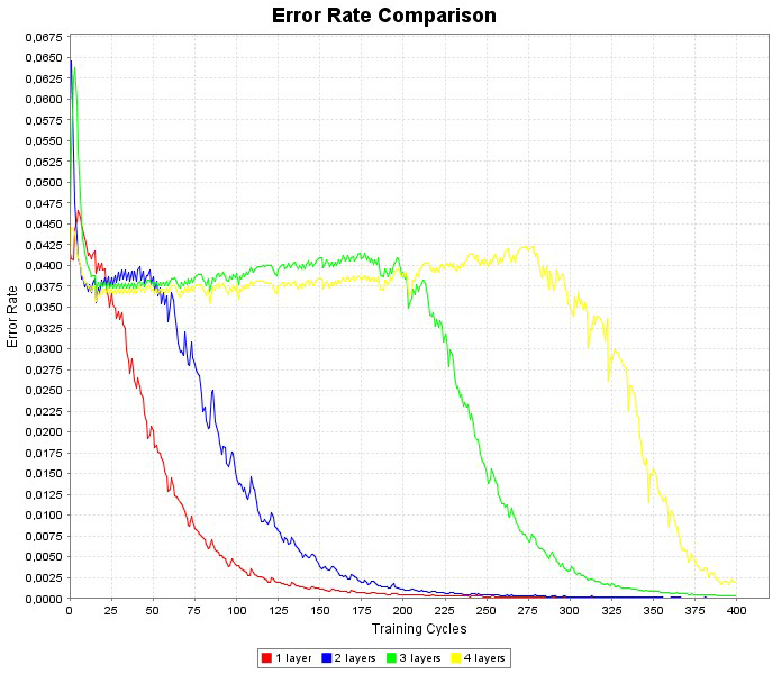
\includegraphics[width=0.7\columnwidth]{graphics/Error_hidden_layers}
	\end{center}
	\vspace{-1em}
	\caption{A comparison using 1, 2, 3 and 4 hidden layers}
	\label{error_hidden}
	\vspace{1.5em}
\end{figure}

Since the resulting error rate is not affected and the time needed to train the network increases with every additional layer the WIDS uses one hidden layer.

\pagebreak

	\item [Number of neurons in the hidden layers:] Table \ref{train_neurons} shows that choosing a higher number of neurons in a hidden layer can improve the resulting output of the network. On the other hand each additional neuron increases the time needed. Each test is performed with 10.000 training cycles.

\begin{table}[htbp]
	\vspace{1.5em}
	\begin{center}
		\begin{tabular}{|l|l|l|}
		\hline
		\bf{Neurons}&\bf{Time needed}&{\bf Error rate}\\
		\hline
		9&5.779 sec&2.09958*$10^{-8}$\\
		\hline
		18&9.263 sec&3.2259*$10^{-9}$\\
		\hline
		36&15.953 sec&2.23715*$10^{-9}$\\
		\hline
		72&30.634 sec&7.80079*$10^{-10}$\\
		\hline
		\end{tabular}
	\end{center}
	\vspace{-1em}
	\caption{Time needed to train the network using 9, 18, 36 and 72 neurons}
	\label{train_neurons}
\end{table}

Another test shows that it takes 30 seconds to test the neural network with 50000 packets and 18 hidden neurons. Therefore the WIDS can process 1666 packets per second. Assuming a 16 MBit WLAN and an average packet size of 1500 bytes it would be necessary to process 1333 packets per second in case the network operates at full capacity. That shows that the WIDS is fast enough to be used in a 16 MBit WLAN.

Due to the amount of time needed to train the network and the resulting performance of the test the WIDS uses 18 neurons in the hidden layer.

\vspace{1.5em}

	\item [Learning rate:] \cite{nn_learning_rate} states that "the larger the learning rate ... the larger the weight changes on each epoch, and the quicker the network learns. However, the size of the learning rate can also influence whether the network achieves a stable solution. If the learning rate gets too large, then the weight changes no longer approximate a gradient descent procedure". That means in other words that choosing a good learning rate results in better network performance than just setting it to a high value near $1$.

Figure \ref{error_learning_rates} shows the first 250 training cycles of the WIDS using different learning rates.

\begin{figure}[htbp]
	\begin{center}
		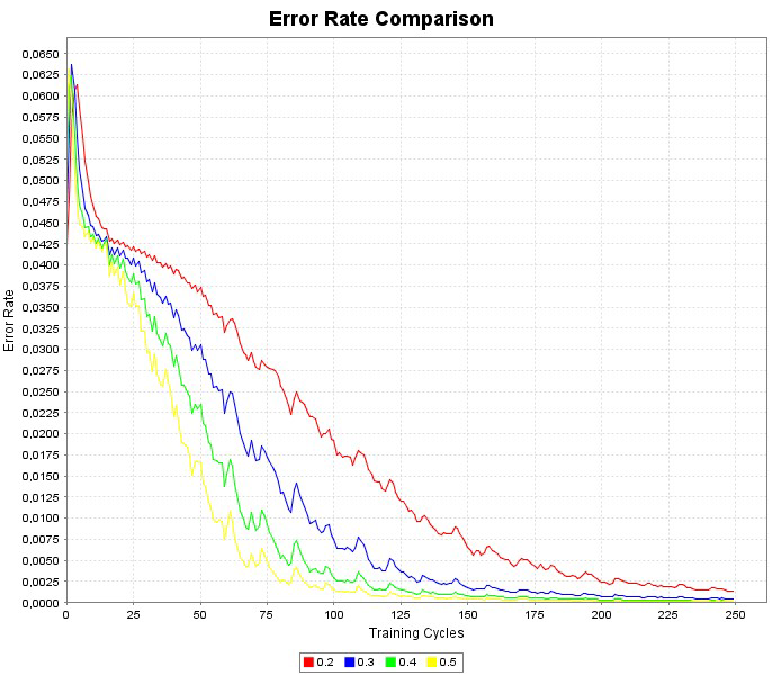
\includegraphics[width=0.7\columnwidth]{graphics/Error_learning_rates}
	\end{center}
	\vspace{-1em}
	\caption{A comparison using 0.2, 0.3, 0.4 and 0.5 as learning rate}
	\label{error_learning_rates}
\end{figure}

On the basis of these results and the warning not to choose a value that is too high the learning rate of the WIDS is set to $0.5$.

\vspace{1.5em}

	\item [Appearance of the sigmoid function:] As shown in figure \ref{error_sigmoid} the value for $a$ in the formula shown in section \ref{sec:activation} provides continuity for the learning process. The result of this test shows that the lower the value $a$ the smaller the difference between two steps in time is. In addition to that, the time needed to train a network increases.

\begin{figure}[htbp]
	\begin{center}
		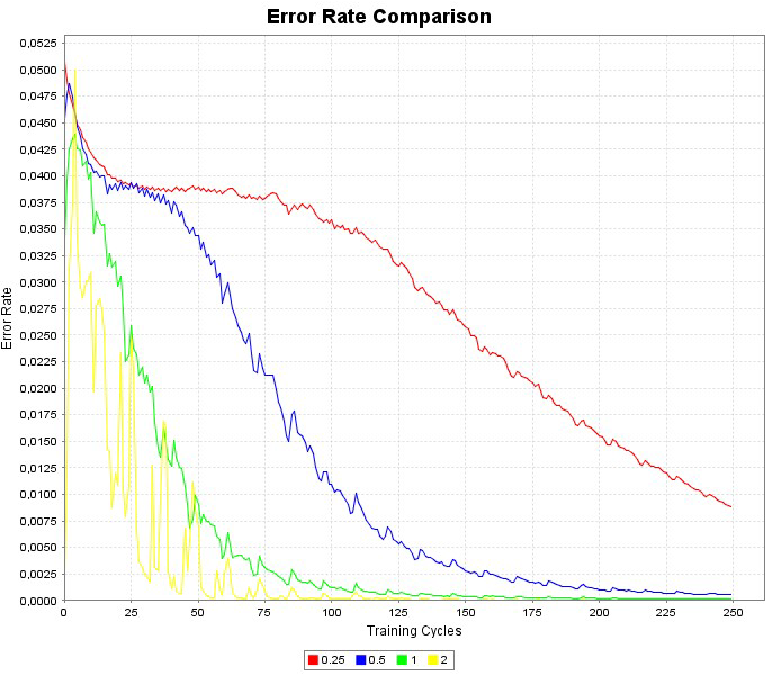
\includegraphics[width=0.7\columnwidth]{graphics/Error_sigmoid}
	\end{center}
	\vspace{-1em}
	\caption{A comparison using 0.25, 0.5, 1 and 2 for the sigmoid function}
\vspace{1.5em}
	\label{error_sigmoid}
\end{figure}

Since one single packet should not affect the obtained result too much and 
in order to avoid a learning process which takes a lot of time the WIDS uses the value of $1$ for $a$.

\end{description}

\section{WIDS}
\label{sec:results_wids}

The following section shows the results obtained by the WIDS. It uses a neural network with the configuration parameters shown in the previous section.

\subsection{Training}

The WIDS is trained by using previously stored pcap files. The characteristics of these files are shown in table \ref{train_env}.

The file in the {\em Normal traffic} column specifies the capture in which no attack occurs. It is a capture of the traffic in a WLAN which is WPA protected. It is created by using a WLAN NIC which is put into monitor mode and the tool Ethereal\footnote{Ethereal is a freely available packet capturing tool. It can be downloaded from http://www.ethereal.com/}.

\begin{table}[htbp]
	\begin{center}
		\begin{tabular}{|l|p{60pt}|p{60pt}|p{75pt}|}
		\hline
		&\bf{Normal traffic}&\bf{Association flood}&\bf{Disassociation flood} \\
		\hline
		Size&9738 KB&21 KB&20 KB\\
		\hline
		Time period&57 sec&9 sec&9 sec\\
		\hline
		Packet count&50000&500&500\\
		\hline
		Associations&5&500&0\\
		\hline
		Disassociations&4&0&500\\
		\hline
		\hline
		Rogue APs&0&0&0\\
		\hline
		Unknown clients&0&500&0\\
		\hline
		Association flood&no&yes&no\\
		\hline
		Disassociation flood&no&no&yes\\
		\hline
		\end{tabular}
	\end{center}
	\vspace{-1em}
	\caption{Properties of the files used for training the WIDS}
	\label{train_env}
\end{table}

The flood files specified in the {\em Association flood} and {\em Disassociation flood} column are created by using a self-made tool\footnote{This tool is named {\em DumpCreator} and is available on the shipped CD}. Both files consist of packets which are used for the respective flood attack only. The association flood uses random source addresses whereas the disassociation flood contains only those MACs as source which are also available in the respective WLAN where the WIDS is used.

\subsection{Testing}

After the training phase is finished the WIDS is tested. Table \ref{result_train} shows the average error values obtained when testing the network with the files used for training shown in table \ref{train_env}.

\begin{table}[htbp]
	\vspace{1.5em}
	\begin{center}
		\begin{tabular}{|l|p{60pt}|p{60pt}|p{75pt}|}
		\hline
		&\bf{Normal traffic}&\bf{Association flood}&\bf{Disassociation flood} \\
		\hline
		No attack&0.999285&0.0158409&0.00934418\\
		\hline
		Association flood&0.000839386&0.981713&0.00531103\\
		\hline
		Disassociation flood&0.00019222&0.00483618&0.988265\\
		\hline
		\hline
		Rogue APs&0&0&0\\
		\hline
		Unknown clients&0&500&0\\
		\hline
		\end{tabular}
	\end{center}
	\vspace{-1em}
	\caption{Average resulting error values using the training files}
	\vspace{1em}
	\label{result_train}
\end{table}

The WIDS identifies normal traffic with almost a 100\% certainty. The different flood attacks are identified with a guarantee of 98\%. Additionally, it detects 500 unknown clients when testing the association flood file since the client's source addresses were created randomly in this file.

The next test is performed with pcap files with the characteristics shown in table \ref{test_env}.

\begin{table}[htbp]
	\begin{center}
		\begin{tabular}{|l|l|l|l|l|}
		\hline
		&\bf{Test 1}&\bf{Test 2}&\bf{Test 3}&\bf{Test 4} \\
		\hline
		Size&9898 KB&10797 KB&10797 KB&10795 KB\\
		\hline
		Time period&65 sec&45 sec&45 sec&45 sec\\
		\hline
		Packet count&50000&50150&50150&50100\\
		\hline
		Associations&2&153&3&53\\
		\hline
		Disassociations&2&2&152&52\\
		\hline
		\hline
		Rogue APs&0&0&2&3\\
		\hline
		Unknown clients&0&149&0&49\\
		\hline
		Association flood&no&yes&no&yes\\
		\hline
		Disassociation flood&no&no&yes&yes\\
		\hline
		\end{tabular}
	\end{center}
	\vspace{-1em}
	\caption{Properties of the files used for testing the WIDS}
	\label{test_env}
\end{table}

The first test file is a capture of the WLAN with similar properties like the file used for training.

The second file is another capture of the WLAN but it also includes MACs of unknown clients and an association flood attack. The flood is performed using 149 association requests of clients with a randomised MAC address.

The third file includes two rogue APs and a disassociation flood. The flood is done by using 150 disassociation requests of legitimate clients.

The last test file contains all types of attacks. It uses 49 association requests and 50 disassociations of legitimate clients. Additionally, it contains 3 rogue APs and 49 unknown MAC addresses.

Table \ref{result_test} shows the results obtained when testing the WIDS using the files shown in table \ref{test_env}. The values in the rows named {\em Association floods} and {\em Disassociation floods} specify the number of feature sets\footnote{One feature set consists of all features described in section \ref{sec:features} and is created for every single packet received.} recognised that identify a specific attack. That means in other words that $0$ indicates that no attack occurs. All values above $0$ mean that one or more feature sets are found which characterise a certain flood attack.

\begin{table}[htbp]
	\vspace{1.5em}
	\begin{center}
		\begin{tabular}{|l|l|l|l|l|}
		\hline
		&\bf{Test 1}&\bf{Test 2}&\bf{Test 3}&\bf{Test 4} \\
		\hline
		Rogue APs&0&0&2&3\\
		\hline
		Unknown clients&0&149&0&49\\
		\hline
		Association floods&0&148&0&48\\
		\hline
		Disassociation floods&0&0&148&48\\
		\hline
		\end{tabular}
	\end{center}
	\vspace{-1em}
	\caption{The resulting numbers of attacks found in the test files}
	\label{result_test}
\end{table}

The test result of the first test file shows the desired result. No malicious activity is found.

In the second test file the WIDS finds the correct number of unknown clients and also detects an association flood. An interesting thing about this result is that the number of feature sets found that identify a flood attack is 148 and not 149. The reason is that the first packet of the flood attack is considered as normal traffic since the number of association packets in the past two seconds is still $0$. This shows that the WIDS alerts a flood attack in case the number of association packets received in a two second time slot exceeds $1$.

The results of the third test files show that the WIDS detects a disassociation flood attack in case the number of disassociations of legitimate clients in the past two seconds exceeds the value $2$. Again, the reason is that the first two disassociations of the attack are considered as valid. In addition to the flood attack both rogue APs are detected correctly.

The result of the fourth test file shows that the WIDS detects all attacks that occur in the network.

\chapter{Conclusion}

\section{Neural Networks for Intrusion Detection}

The results shown in section \ref{sec:results_wids} indicate that a neural network can be used efficiently in an intrusion detection system. A big advantage of using a neural network lies in the fact that the IDS can react to changes in the network characteristics.

Another important aspect is the preciseness of the system. If the characteristics in a WLAN do not change over time and the attacks are performed with enough packets the IDS detects all occurring association and disassociation flood attacks as well as malicious clients and rogue APs.

On the other hand there exist some drawbacks that an IDS developer needs to think of: Due to the complex structure of the neural network it is necessary to provide enough memory and computing power. Especially the training phase takes a lot of time depending on the amount of available data. Additionally, the network links between the data gatherer(s) and the data processor need to be faster than the speed in the WLAN network itself.

\section{Neural Networks and Traditional Methods}

\cite{nn_vs_traditional} poses the question whether it is better to use neural networks or traditional techniques\footnote{Traditional techniques in this context mean an anomaly based IDS which does not use a neural network. See section \ref{sec:sig_anom_ids} for details} to solve certain problems. The answer is that this is "an unanswerable question" \cite[p.4]{nn_vs_traditional}. The main problem lies in the characteristics of ANNs:

First, the weight values that are used to setup an uninitialised network are chosen randomly. This means the obtained results differ slightly each time the network is trained even if the same training set is used.

Next, as described in section \ref{sec:features}, the success of learning something is highly dependent on the features chosen for the input nodes. As a consequence the quality of the results differs significantly if different features are chosen.

Finally, the architecture and properties of the neural network itself change the results obtained. Section \ref{sec:test_nn} shows that depending on the number of hidden layers and neurons the performance of the network varies.

\section{Future Work}

The following section discusses tasks that need to be done before using the WIDS and possible improvements which make the WIDS more powerful.

\subsection{Putting the WIDS into a Real Network}

All tests have been done by using previously stored pcap files. The next step, to improve the WIDS, is to train it and put it in a WLAN to find out whether it behaves correctly and whether it reacts to changes in the network behaviour. This can only be done by running the WIDS over periods of several weeks and months.

Additionally, it is important to find out whether the neural network is fast enough to process the incoming traffic in real time or whether it is necessary to preprocess the traffic. In case the amount of traffic is too large for the neural network to handle it would be interesting to know how fast the WLAN may be until the WIDS can not process the data any longer.

\subsection{Adding Remote Functionality}

As described in section \ref{sec:design_wids} the design of the WIDS makes it possible to create remote sensors which collect data in a WLAN and send it to the data processor. As a consequence the data gathering component needs to be realised as a stand alone tool which connects to the data processor: The data processor is the server which waits for incoming data packets. Currently the WIDS does not support this form of client/server architecture.

\subsection{Adding Silent User Detection}

If a malicious user is present in a network but not sending any packets, it is impossible for the WIDS to detect this client because it needs packets to work with. As a consequence it is necessary to extend the WIDS with the capability to send RTS packets. As described in section \ref{sec:hidden_node_problem} the RTS/CTS handshake is used to overcome the hidden node problem. The answer to the RTS packet, the CTS frame, is sent automatically. This means that it is not possible (at least with unmodified hardware) to prevent the sending of a CTS packet. The RTS/CTS handshake makes it possible to detect clients although they do not send packets.

A drawback of this method is that a client needs to be known as malicious because it is necessary to know the MAC address to which the RTS packet is sent to.

\subsection{Adding Scanner Fingerprinting}

As described in \cite{wlan_fingerprints} some active wireless scanners like Netstumbler or Wellenreiter provide individual characteristics when they send frames. That makes it possible to find out what type of scanner an intruder is using.

\subsection{Reacting on Intrusions}

Currently the WIDS writes an alert message on the screen whenever a flood attack is recognised or an unknown MAC address is found. The next step is to react to possible threats automatically. Possible counter measures include modifying the firewall to block a certain client or to send a mail to the network administrator to inform about ongoing threats.

\subsection{Providing a GUI}

Currently the WIDS alerts the user by printing a message on the screen. It would be easier to configure and handle this tool if it is based on a GUI. It could consist of a configuration section which is capable of changing the structure of the neural network. Additionally, it should be possible to perform the training and testing phase of the WIDS graphically.

\section{Outlook}

As explained in \cite{IDS_terminology} "Intrusion Detection Systems (IDS) are still in their infancy" and as a consequence used very rarely. On the other hand it is a very fast evolving area in computer science.

The underlying work shows that using a neural network can be advantageous and will very likely find its way in upcoming (wireless) intrusion detection systems.
